\section{Method}

% \lau{Lau: As far as I'm concerned, everything below before subsection 2.1 could also go at the end of the Introduction. Beyond the fact that it contains literature review and conceptual information that would go well in the intro, I find the current architecture of Section 2 a bit puzzling. First there is text to explain the methods and detail their intuition/key components, then there are three consecutive subsections that kind of do the same, but from a maths points of view. The aforementioned suggestion of putting the first text in the intro could solve this. Another possibility: put the descriptive texts in their corresponding sub-sections, so that those contain both the motivation and the maths. I'm open to further suggestions and suggestions ;-) }
% \mdeff{Indeed. The "Distance Learning" and "Orientation Recovery" paragraphs might go in their respective sub-sections. But I'd like to keep a high-level motivation of the whole method (the text linked to the second figure to appear alongside \figref{imaging-geometry}.} \lau{Fine for me.}\banjac{I moved the DE and OR to corresponding subsections. The short intro to methods I left here at the beginning of the section 2 (I didn't move it to intro). Let me know if you meant something different}

\begin{figure}
    \centering
    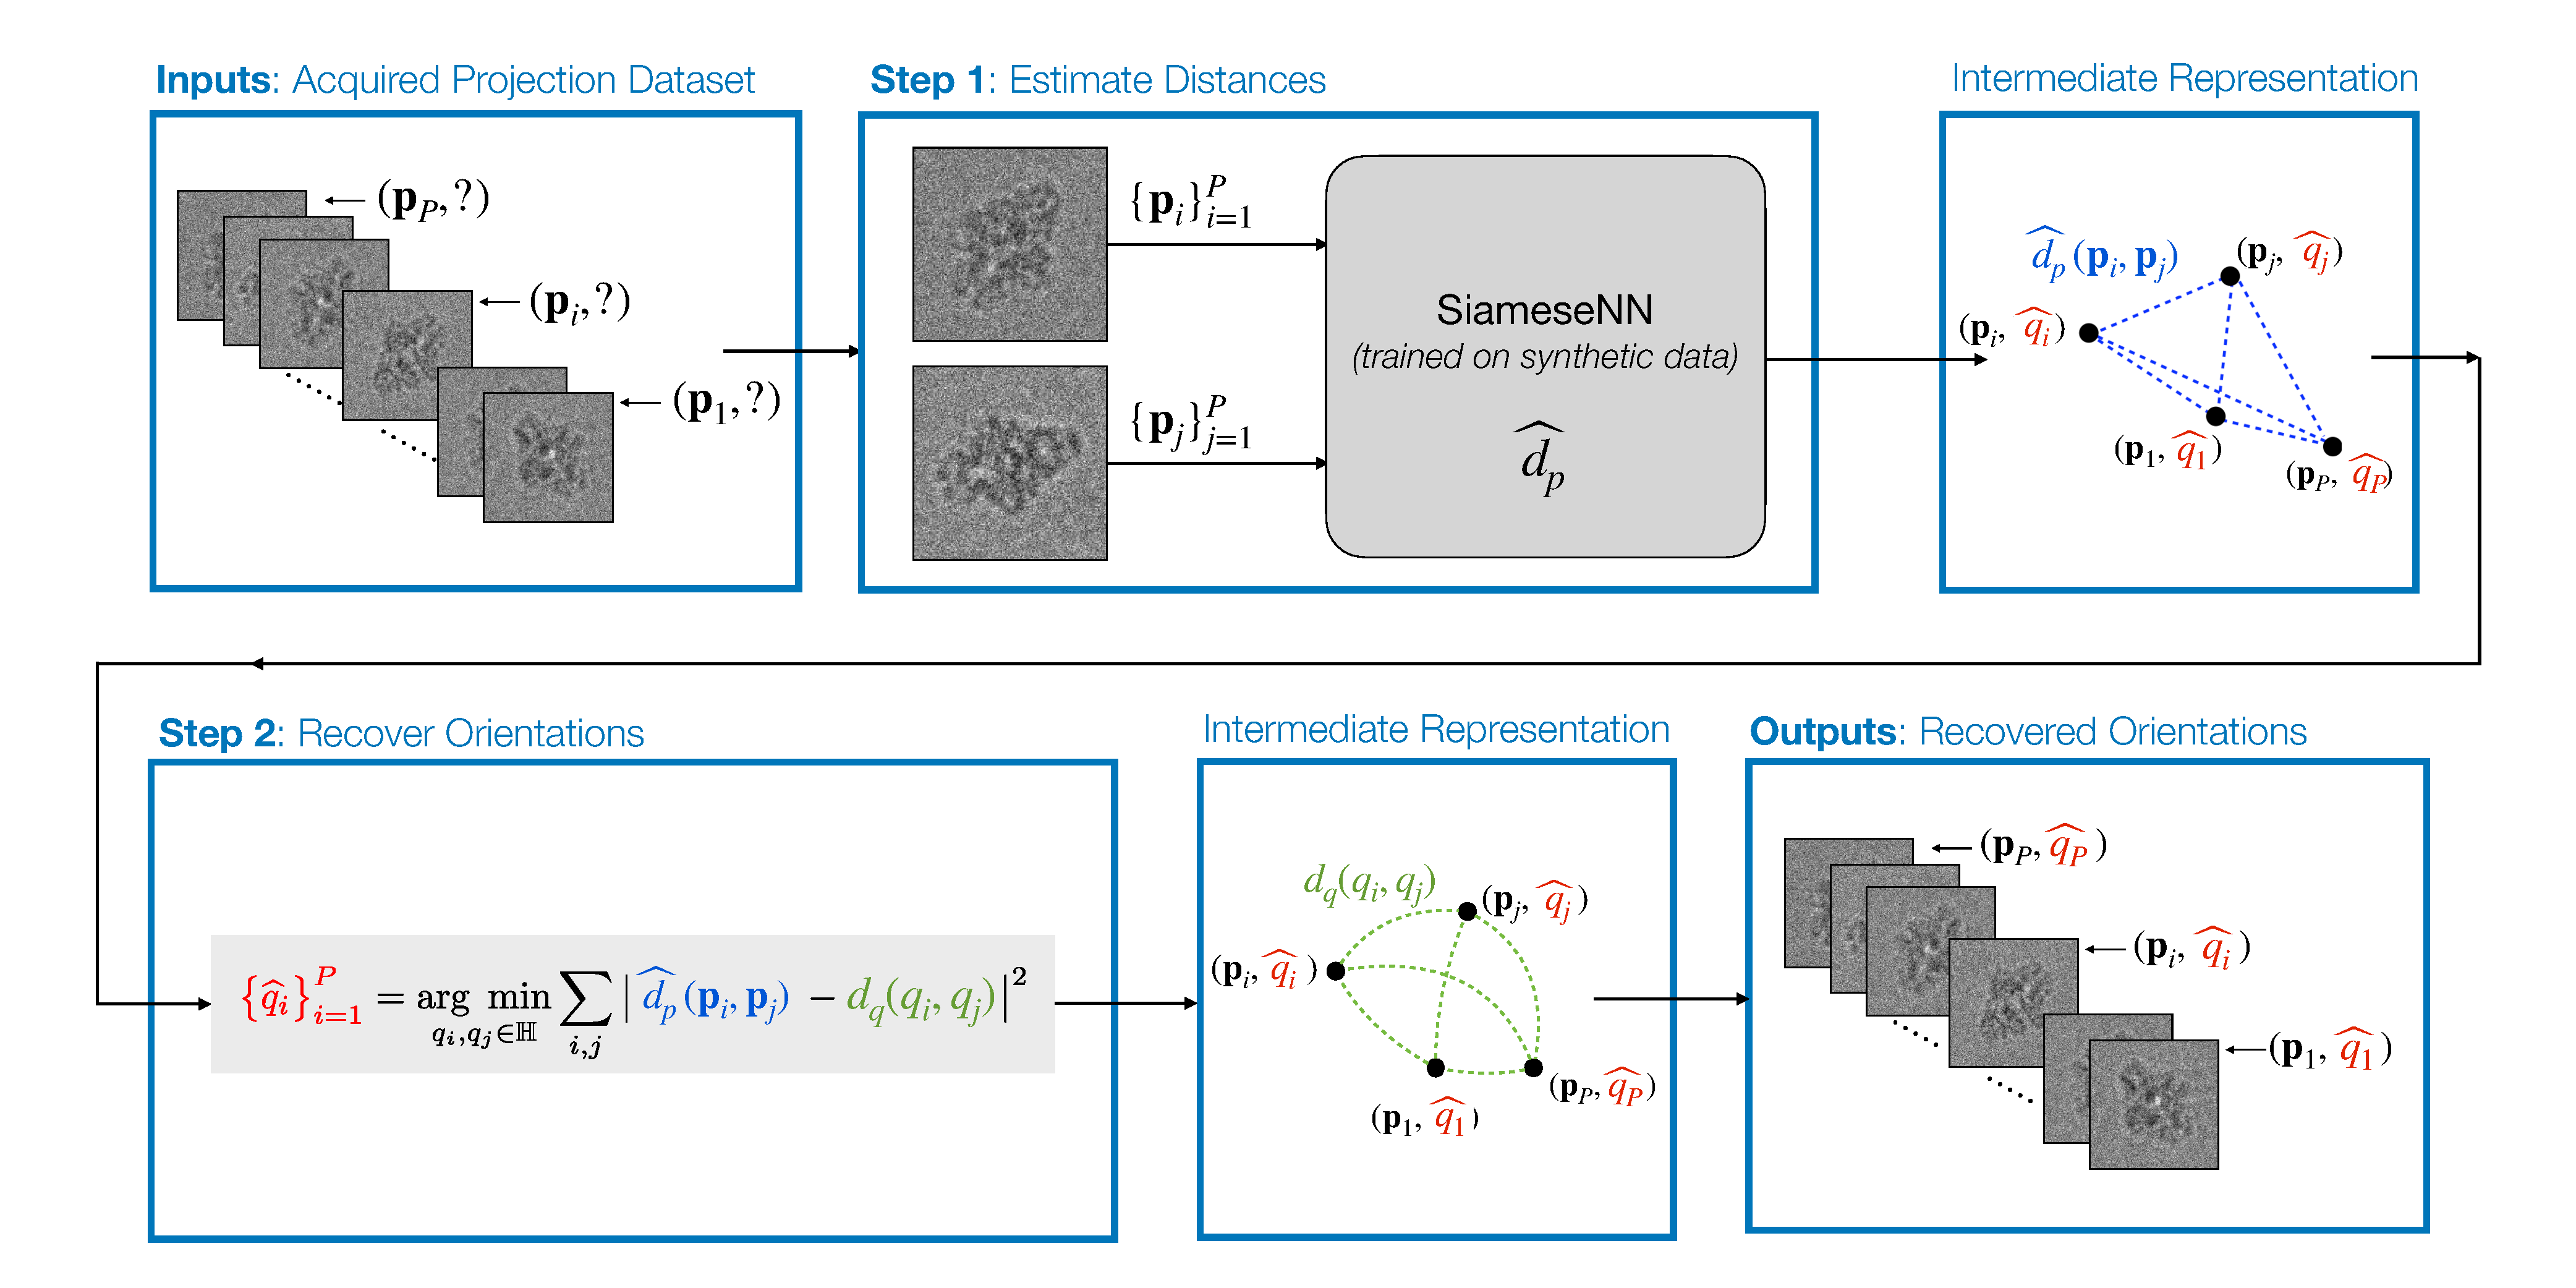
\includegraphics[width=\textwidth]{schematic_method_overview}
    \caption{
        \textbf{Method overview.}
        We denote the $i$th projection by $\mathbf{p}_i$ and its orientation by $q_i$. The distance between two orientations is denoted by $d_q$, and the estimated distance between two projections by $\widehat{d}_p$; the latter is implemented as a SiameseNN.
        Our method consists of two steps: (i) estimate distances between pairs of projections, and (ii) recover orientations from the estimated distances.
        % Our method effectively (i) estimates a metric space, then (ii) embed/realize it in the space of 3D orientations, $\SO(3)$.
        % \todo{Update sections in figure.}
        % \todo{Update titles: Step 1: estimate distances. Step 2: recover orientations.}
        % \mdeff{It would be amazing to have a visual of the embedding made in step 2: finding points in SO(3) such that the geodesic distances between them are the estimated distances. As we can't see SO(3) / $S^3$, we could try with $S^2$, which is a subset/projection.} \lau{I'll change the notations in the figure once we have settle on the final ones.}
    }\label{fig:schematic:method-overview}
\end{figure}

We present a method that learns to estimate the unknown orientation associated to each projection in a single-particle cryo-EM dataset without relying on any intermediate reconstruction procedure. Our approach relies on the well-know observation that the greater the similarity between two 2D projections, the more likely they originated from two 3D particles that adopted close orientations in the ice layer prior to imaging;\footnote{Up to protein symmetries, which we discuss later.} this principle guides a number of applications in the field~\cite{frank2006three}.

Taking this line of thought further, we propose to train a function---parametrized as a neural network---to predict the relative orientation between two projections based on their similarity. This trained network then allows us to estimate, for any new projection dataset, the relative orientations between pairs of its projections. From these estimated distances, we then retrieve the orientation for each projection through an appropriate minimization scheme. Our two-steps method is illustrated in \figref{schematic:method-overview}.

%to embed it on the space of 3D orientations, $\SO(3)$.
% In practice, our method consists of: (i) estimate the distance between pairs of projections, and (ii) recover
% \mdeff{maybe too repetitive with figure caption}

% Note; here was Distance Learning. paragraph

%If the distances are exact geodesic distances between orientations, then orientation recovery will find a perfect realization of the metric space, with zero error.
%In practice, distances estimated from projections will only be a proxy of true distances.
%Experiment \secref{results:orientation-recovery:sensitivity} shows that a lower distance estimation error translates to a lower orientation recovery error.

% Note; here was Orientation Recovery. paragraph

%%%%%%%%%%%%%%%%%%%%%%%%%%%%%%%%%%%%%%%%%%%

%\subsection{Unit Quaternions and the Geodesic Distance}
%\subsection{Parameterization of orientations}
\subsection{Representation of orientations}\label{sec:method:orientation-representation}
%\mdeff{Laurène: Which word is better: Representation or parameterization? Or something else, but we need consistency.} \lau{Both are fine. Personally, I use parametrization in my thesis, but we can settle on the other one.}

Inside the electron microscope, each 3D particle is positioned at a given orientation with respect to the detector plane $\bsy=(y_1,y_2)\in \mathbb{R}^2$, as illustrated in \figref{imaging-geometry}.
Hence, for each particle, the geometry of the imaging procedure is described by the geometrical transformation that maps its object coordinate system $(x_1,x_2,x_3)$ to the measurement coordinate system $(y_1,y_2)$. 
This mapping corresponds to an integration through the 3D particle according to the orientation.
As opposed projections are mirrored, we cannot resolve chirality\footnote{A geometric property which says that the mirror transformation of an object is a non-identity operation, i.e. the object and its mirror image cannot be aligned by any translation or rotation.}. 
Projecting looses global orientation, and integrating looses chirality.



There is a variety of representations of orientations used in practice. Bellow we note the advantages and disadvantages for each of them.

\paragraph{Euler angles.} The standard approach in single-particle cryo-EM is to use Euler angles to parametrize the rotation matrix that relates the two coordinate systems~\cite{sorzano2014interchanging}.
The Euler angles, denoted as $\bth = (\theta_3,\theta_2,\theta_1) \in [0,2\pi[ \, \times \, [0,\pi] \times [0,2\pi[$, are a set of three angles in angle space that describe a sequence of three rotations about three fixed axes. In cryo-EM the most widely used convention is $Z3-Y2-Z1$. 
First, we rotate about $Z1$-axis ($\theta_1$ is called a rotation angle). 
Then. we rotate about $Y2$-axis ($\theta_2$ is called an azimuthal or tilt angle). 
Lastly, we rotate about $Z3$-axis ($\theta_3$ is called in-plane rotation).
In general, Euler angles are not unique and they suffer from \textit{gimbal lock} problem\footnote{The gimbal lock problem arises when $\theta_2=0$ and restricts the number of rotational degrees of freedom to one even though $\theta_1$ and $\theta_3$ have not yet been fixed~\cite{koks2006explorations}.}.
Compared to other representations, they use the least memory (3 scalars). 
The projection direction is determinded only by two angles, $\theta_1$ and $\theta_2$. However, to compare whether two different projections are close to each other in their projection directions (i.e. their geodesic distance is small), it cannot be directly computed from their two sets of Euler angles. 
% Euler angles:
% - Euler angles are not unique
% - gimbal lock problem
% - intuition behind changing the basis between two coordinate systems is not so clear
% - to compare if 2 different projs are close to each other in their projection direcitons, it does not suffice comparing their 2 sets of Euler angle sets
% - 3 unkown parameters
% - just used for representation of input and output format of rotation


\paragraph{Rotation matrices.} One way to compute the geodesic distance between two projection directions is to represent orientations as rotation matrices. Mathematically, we write $\mathbf{R} = \mathbf{R}_{Z3}(\theta_3) \mathbf{R}_{Y2}(\theta_2) \mathbf{R}_{Z1}(\theta_1)$, where $\mathbf{R},\mathbf{R}_{Z3}(\theta_3),\mathbf{R}_{Y2}(\theta_2), \mathbf{R}_{Z1}(\theta_1) \in \SO(3)$. 
Hence, the orientation is defined as a rotation in $\SO(3)$ space, the group of all 3D rotations about the origin of $\mathbb{R}^3$ under the operation of composition (i.e. order of rotations matter); in that space, every rotation can be described by a $3\times3$ orthogonal matrix with determinant~$1$.
The rotation matrices are intuitive in the 3D space transformations. 
They support versatility of transformations -- besides rotation they support reflections, translations, scaling, etc. 
Unlike Euler angles, rotation matrices avoid gimbal lock. 
However, they are computationally more expensive since we are dealing with $3\times3$ matrices (i.e. 9 scalars).
% Affine transformation
% - intuitive
% - unique (and for each rotation matrix there is a unique quaternion with norm 1)
% -  3x3 matrix, 9 parameters
% - used when angle alignment was performed due to its transformation versatility (e.g. supports mirrors)
% simpler to compose
% avoid problem of gimbal lock

\paragraph{Quaternions.} Unit quaternions $q \in \U$, with  $\U = \big\{ q \in \mathbb{H}: \lvert q \rvert = 1 \big\}$, which identifies the $\mathbb{S}^3$ hypersphere in $\R^4$ are another way of representing the 3D rotations.
Unit quaternions represent rotations as $\mathbb{S}^3$ is a double-cover of $\SO(3)$, i.e. mapping from unit  quaternion to $\SO(3)$ is 2-to-1, $\mathbf{R}(q) = \mathbf{R}(-q)$ (antipodal points are identified).
You can find the necessary background on quaternions in Appendix~\ref{sec:quaternions}.
Quaternions are used in the cryo-em to a lesser extent. 
Unfortunately, the intuition behind changing the basis between two coordinate systems is not so clear and performing reflections (also known as mirrors, flips) using quaternions we lose any intuition about how two projection directions (mirrored and non-mirrored) are related. 
However, quaternions are more compact (4D vectors/4 scalars) and numerically stable compared to rotation matrices. 
The quaternions strike a nice balance of both, Euler angles and rotation matrices, being small and free from gimbal lock.

As our method requires the repeated computation of the geodesic distance, we resort to a more convenient representation of 3D rotations that relies on unit quaternions.
The geodesic distance between two orientations, i.e. the length of the geodesic between them on the surface of $\SO(3)$, is defined as
\begin{equation}
    \begin{array}{c}
    d_q: \U \times \U \rightarrow [0,\pi],\\
    d_q(q_i, q_j) = 2 \arccos \big(| \langle q_i, q_j \rangle| \big),
    \label{eqn:distance:orientations}
    \end{array}
\end{equation}
with $\langle q_i, q_j \rangle$ the inner product between two quaternions~\cite{huynh2009metrics}. As $\mathbb{S}^3 = \{x \in \R^4: \left\Vert x \right\Vert\ = 1\}$ is isomorphic to the universal cover of $\SO(3)$, $d_q$ corresponds to the magnitude of the rotation $\mathbf{R}_* \in \SO(3)$ such that $\mathbf{R}(q_i) = \mathbf{R}_* \mathbf{R}(q_j)$~\cite{huynh2009metrics}.
In other words, the distance between two rotations represented as unit quaternions can be efficiently computed from the quaternions themselves.
% Quaternions:
% - intuition behind changing the basis between two coordinate systems is not so clear
% - 4D vector, 4 unknown parameters
% - much less known in EM community, but they can be used to describe rotation
% - any time we need to perform rotation on camera position, the quaternion is translated into its corresponding rotation matrix and then it is applied to the coordinates of the central coordinate system
% - mirroring using quaternions - we lose any intuition about how two projection direcitons (mirrored and non-mirrored) are related
% more compact and numerically stable

% Axis angles 
% - used for visualizations

%Note that all of these representations of rotations are used in practice. Euler angles use the least memory; matrices use more memory but don't suffer from Gimbal lock and have nice analytical properties; and quaternions strike a nice balance of both, being lightweight, but free from Gimbal lock.
%Rotation matrix: Minor disadvantage: Multiplication of matrices is ~2 times slower than quaternions. Minor Advantage: Matrix-vector multiplication is ~2 times faster, and large. Huge disadvantage: Normalization! Ghram-Shmit is asymmetrical, which does not give a higher order accurate answer when doing differential equations. More sophisticated methods are very complex and expensive.
%Axis (angle = length of axis) Minor advantage: Small. Moderate disadvantage: Multiplication and applying to a vector is slow with trig. Moderate disadvantage: North-pole singularity at length = 2*pi, since all axis directions do nothing. More code (and debugging) to automatically rescale it when it gets near 2pi.


%\mdeff{Not only a rotation, but an integration through $z_3$. (As opposed projections are mirrored, we cannot resolve chirality. Projecting looses global orientation, integrating looses chirality.)}


%As our method requires the repeated computation of the geodesic distance, we resort to a more convenient representation of 3D rotations that relies on unit quaternions $q \in \U$, with  $\U = \big\{ q \in \mathbb{H} \; \, | \; \, \lvert q \rvert = 1 \big\}$, which identifies the $\mathbb{S}^3$ hypersphere in $\R^4$.
%and concisely represent the elements of the $\SO(3)$ group.
%\todo{Better transition from quaternions to rotations.}
%Unit quaternions represent rotations as $\mathbb{S}^3$ is a double-cover of $\SO(3)$, i.e., $\mathbf{R}(q) = \mathbf{R}(-q)$ (antipodal points are identified).
%You can find the necessary background on quaternions in Appendix~\ref{sec:quaternions}.

%through~\eqnref{distance:orientations}, which is of key practical importance for this work.

%For the sake of conciseness, we shall use the term ``with orientation~$q$'' to refer to 2D/3D objects considered in an imaging geometry parametrized by $q$.

%%%%%%%%%%%%%%%%%%%%%%%%%%%%%%%%%%%%%%%%%%%

\subsection{Distance learning}\label{sec:method:distance-learning}
%\subsection{Metric learning}%\label{sec:method:distance-learning}
%\subsection{Estimating Relative Orientations from Projections}
%\subsection{Relative orientation estimation}
%\subsection{Relative orientation estimation from projections}

%We capitalize on the powerful function approximation capabilities of neural networks and on our ability to faithfully model the cryo-EM imaging process for the generation of training data.

%To make such training possible, we capitalize on our ability to model the cryo-EM imaging procedure to generate a large, representative synthetic dataset using publicly available 3D atomic models.
%Once the distance learned, it can be used in the aforementioned two-steps method (see \figref{schematic:method-overview}) for any projection dataset.

%\paragraph{Distance Learning.}
The resort to a neural network to estimate the relative distances is driven by several reasons. First, and most obviously, this information is not directly accessible from the dataset itself. To circumvent this, we rely on the postulate that the similarity between two projections is a good proxy for their relative orientation, for some appropriate meaning of similarity. The ``handcrafting'' of a metric that would robustly predict these distances is an intricate---if not impossible---task, partly because the invariants are difficult to specify. Hence, we rather opt to \textit{learning} this distance function by parameterizing it as a neural network. For its training, we capitalize on (i) the public availability of numerous 3D atomic models\footnote{\url{https://www.ebi.ac.uk/pdbe/emdb}} and (ii) our ability to model the cryo-EM imaging procedure in order to generate realistic cryo-EM projection datasets.

The goal is to train a function---parametrized as a neural network---to predict the relative orientation between two projections based on their similarity. \figref{schematic:distance-learning} illustrates the proposed learning paradigm.

\begin{figure}
    \centering
    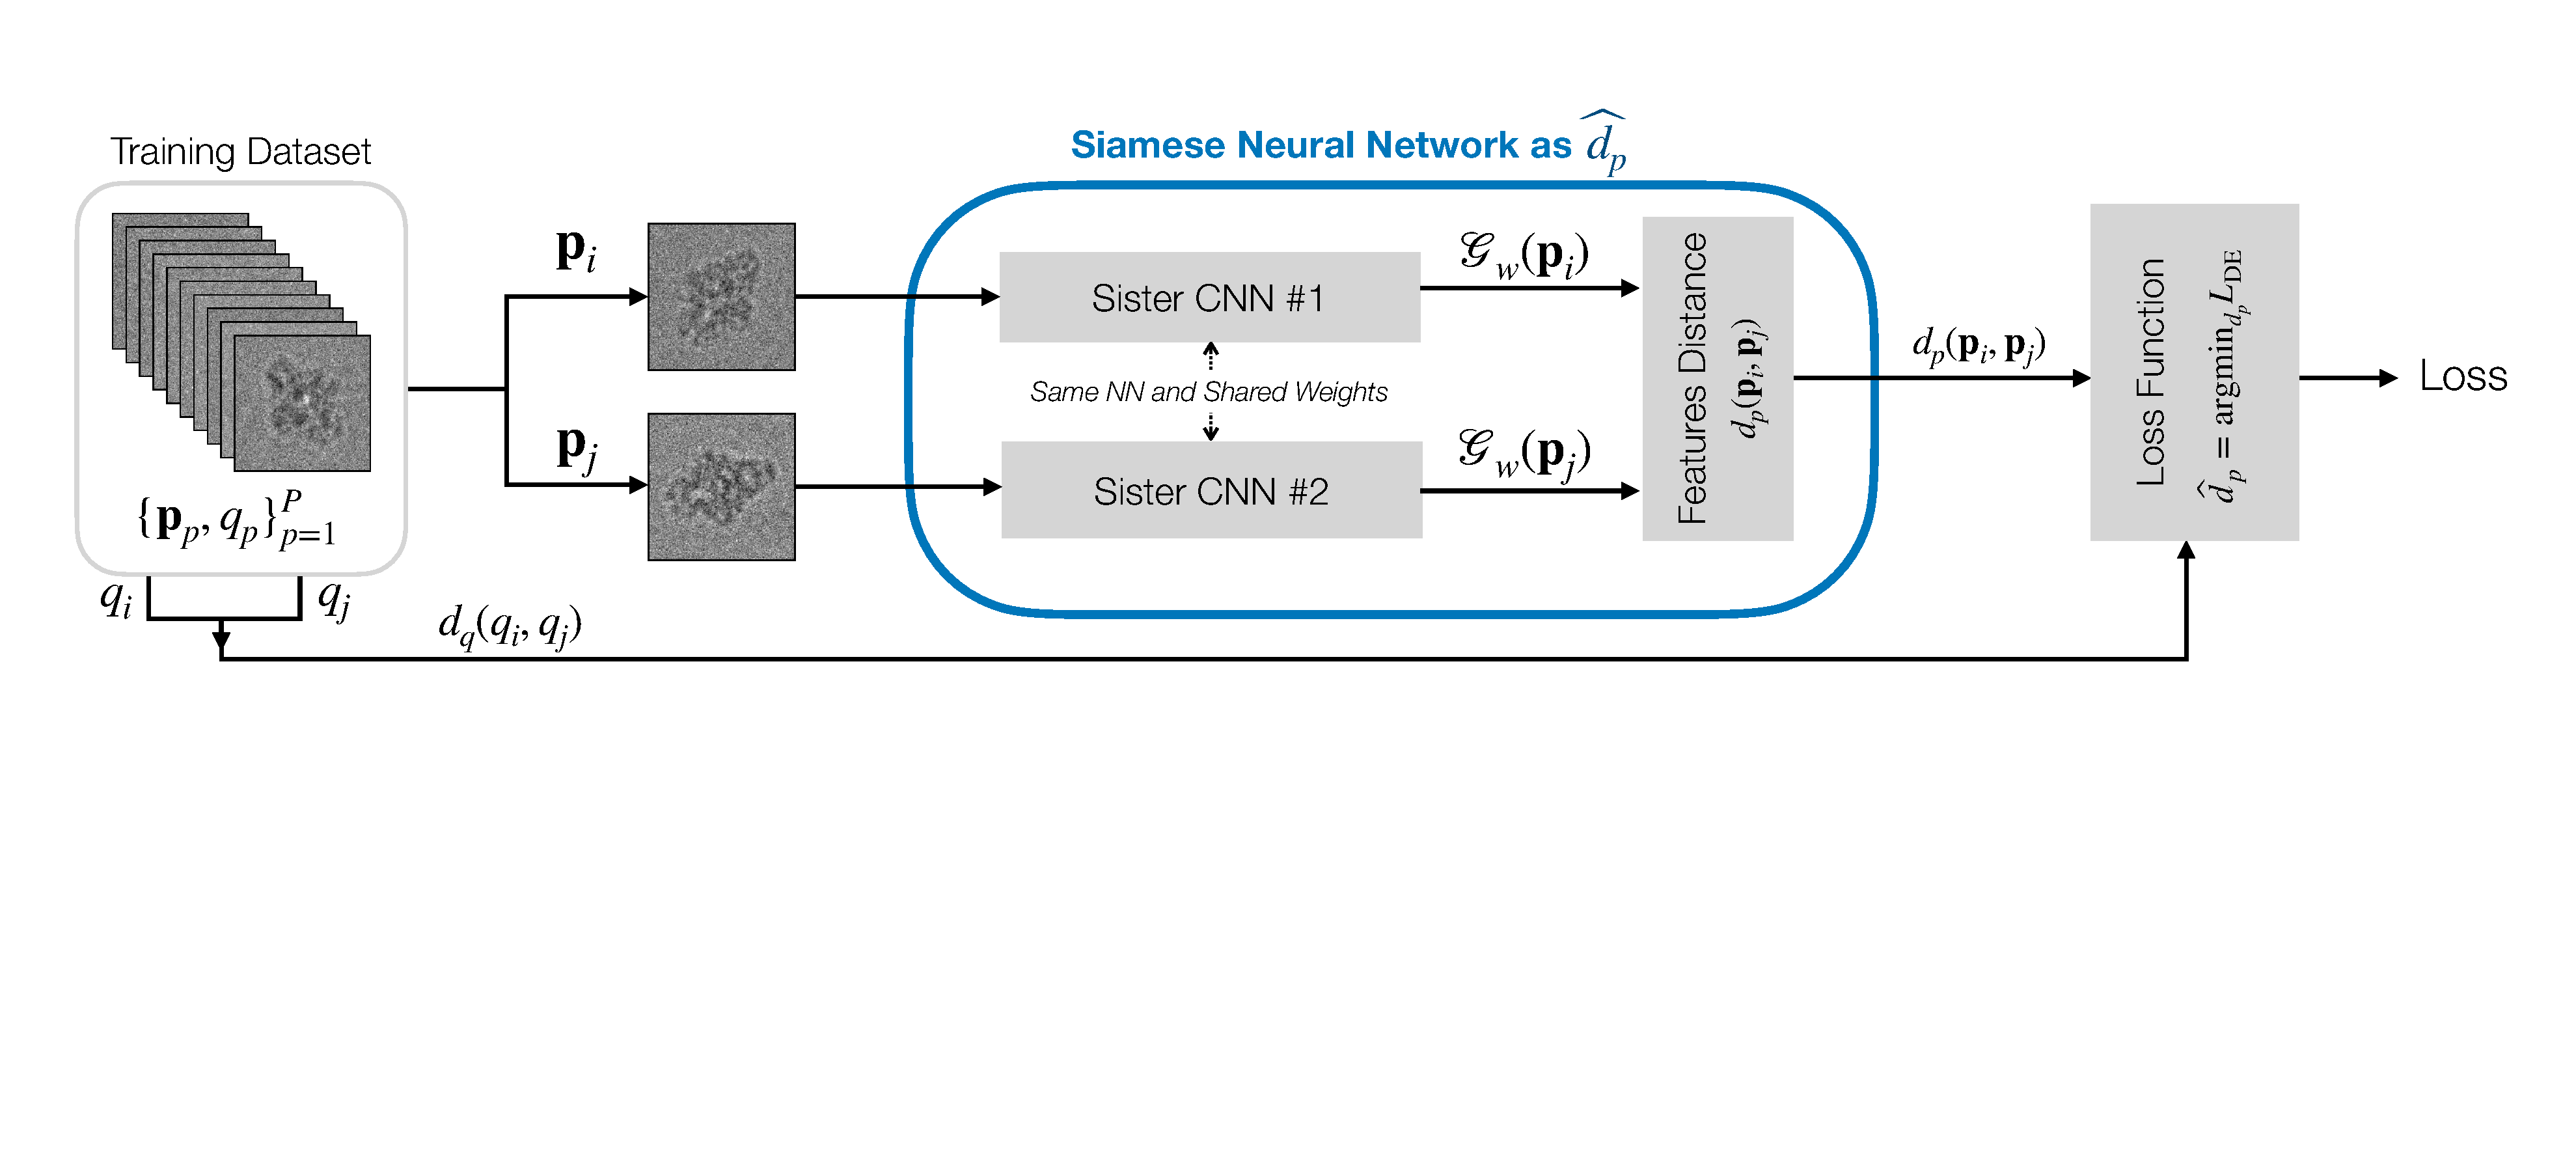
\includegraphics[width=\textwidth]{schematic_distance_learning}
    \caption{%
        We are looking for a distance $d_p$ between projections that is an accurate estimator of the distance $d_q$ between their orientations.
        We propose to parameterize $d_p$ as a Siamese neural network (SiameseNN), trained on a synthetic dataset of $P \approx 10^3$ projections with associated orientation.
        %\todo{Figure: feature distance (not similarity) $d_f$ is \eqnref{distance:projections}. Loss function is \eqnref{distance-learning}. "Same Structure/Weights" $\rightarrow$ "Same NN $\G$ and shared weights $w$".}
}\label{fig:schematic:distance-learning}
\end{figure}

From a training dataset ${\{ \mathbf{p}_{i}, q_i \}}_{i=1}^{P}$ made of $P$ projections $\p_i \in \R^{n_p}$ with associated orientation $q_i \in \U$, we learn the \textit{projection distance}
\begin{equation}
    \widehat{d}_p = \argmin_{d_p} \sum_{i,j} \left| d_p\big(\mathbf{p}_{i},\mathbf{p}_{j}\big) - d_q\big(q_i,q_j\big) \right|^2,
    \label{eqn:distance-learning}
\end{equation}
with $d_q$ defined in~\eqnref{distance:orientations}.
The distance $d_p$ is parameterized as the Siamese neural network (SiameseNN)~\cite{chopra2005learning}
\begin{equation}
    d_p(\p_i, \p_j) = d_f(\G_w(\p_i), \G_w(\p_j)),
    \label{eqn:distance:projections}
\end{equation}
where $\G_w$ is a convolutional neural network with weights $w$ that is trained to extract the most relevant features $\f_i \in \R^{n_f}$ from a projection $\p_i$. SiameseNNs, also termed ``twin networks'', are commonly used in the field of deep metric learning to learn similarity functions~\cite{yi2014deep}.
The distance in the feature space $d_f$ is often taken to be the Euclidean distance $d_f(\f_i, \f_j) = \Vert \f_i - \f_j \Vert_2$.
To facilitate the learning of a distance that respects the elliptic geometry of $\U$, we set $d_f = d_q$.

Evaluating the sum in \eqnref{distance-learning} has complexity of $\mathcal{O}(P^2)$ since we have $\frac{P^2-P}{2}$ distance evaluations.
As this is computationally intractable for cryo-EM datasets with typically $P \approx 10^5$ projections, we sample only a subset of pairs.
In practice, \eqnref{distance-learning} is minimized by stochastic gradient descent (SGD) over small batches of pairs, with weight updates computed by back-propagation of the error.
% error / objective value

%%%%%%%%%%%%%%%%%%%%%%%%%%%%%%%%%%%%%%%%%%%

\subsection{Orientation recovery}\label{sec:method:orientation-recovery}
%\subsection{Orientation recovery from relative orientations}

%\paragraph{Orientation Recovery.}
The task of recovering points based on their relative distances has been extensively studied in the literature, primarily within the frameworks of dimensionality reduction and data visualization~\cite{belkin2003laplacian,kruskal1978multidimensional, maaten2008visualizing, mcinnes2018umap,dokmanic2015euclidean}.
These methods aim at mapping high-dimensional data onto a lower-dimensional space in such a way that the structure of the metric space is preserved.
Formally, the recovery is achieved by minimizing an appropriate loss function; well-known examples include Laplacian eigenmaps, multi-dimensional scaling (MDS), Isomap, LLE, t-SNE, and UMAP.
In the Euclidean setting, the embedding of distance matrices (given by their eigenvectors) is especially well-described.
In particular, the framework of the Euclidean distance matrices (EDMs)~\cite{dokmanic2015euclidean} provides theoretical guarantees on the retrieval of points from collected distances.

In our case, as we shall shortly explain, we aim to perform the embedding on $\SO(3)$, the non-Euclidean space of 3D rotations. Hence, the loss function to minimize (\secref{method:orientation-recovery}) is non-convex. Furthermore, we are not aware of any theoretical characterization of its behavior when input distances are lacking or corrupted by perturbations. That being said, the locally-Euclidean behavior of the $\SO(3)$ space offers some hope on the feasibility of this minimization.
Indeed, despite the lack of theoretical guarantees, we are able to appropriately minimize our loss function using a gradient-based algorithm, as we experimentally demonstrate in \secref{results:orientation-recovery:exact}.

Equipped with a trained estimator $\widehat{d}_p$, we then recover the orientations from a set of projections $\big\{ \mathbf{p}_k \big\}_{k=1}^P$ through
\begin{equation}
    \big\{ \widehat{q}_k \big\}_{k=1}^P = \argmin_{q_i, q_j \in \U} \sum_{i,j} \left| \widehat{d}_p \left( \p_i, \p_j \right) - d_q\left(q_i,q_j\right) \right|^2.
    \label{eqn:orientation-recovery}
\end{equation}
Note that the sole difference with~\eqnref{distance-learning} is that the minimization is performed over the projections $q_i$ rather than the distance $d_p$. 
Here again, the sum in \eqnref{orientation-recovery} is sampled for computational reasons.

A strategy, commonly employed by methods for sparse embedding like multidimensional scaling (MDS), Isomap, etc.~\cite{platt2004fast, 5438584,DBLP:journals/corr/abs-1811-10470} that amounts to build and embed a sparse distance graph. 
More specifically, these algorithms take a matrix of distances and find vectors in a lower dimensional space that well match the inter-vector distances.
Hence, it is possible to determine the coordinates in a lower dimensional space only by knowing their pair-wise distances (at least in Euclidean space).
In our work, we are dealing with non-Euclidean space and we show that it is also possible to determine the coordinates in a lower dimensional space (quaternion space) knowing only the learned pair-wise geodesic distances between two projections.
%\lau{@Mdeff: Can you please fill here? Thanks.}
In practice, \eqnref{orientation-recovery} is also minimized by mini-batch SGD.
%We experimentally demonstrate in \secref{results:orientation-recovery:exact} that both approximations don't affect recovery performance.
